%% A brief test of different estimators of galaxy peculiar velocity
%% Sun Nov 29, 2015
%% Christopher Rooney

\documentclass[usenatbib]{mn2e}
\nonstopmode
%%%%%%%%%%%%%%%%%%%%%%%%%%%%%%%%%%%%%%%%%%%%%%%%%%%%%%%%%%%%%%%%%%%%%%
%% This section is called the preamble, where we can specify which
%% latex packages we required.  Most (but not of all) of the packages
%% below should be fairly standard in most latex documents.  The
%% exception is xspace and the new \latex command, which you probably
%% do not need.
%%%%%%%%%%%%%%%%%%%%%%%%%%%%%%%%%%%%%%%%%%%%%%%%%%%%%%%%%%%%%%%%%%%%%%

%% Bibliography style:
\usepackage{mathptmx}           % Use the Times font.
\usepackage{graphicx}           % Needed for including graphics.
\usepackage{url}                % Facility for activating URLs.
\usepackage{verbatim}           % For verbatiminput command.
\usepackage{booktabs}
%% Set the paper size to be letter, with a 2cm margin 
%% all around the page.
\usepackage{gensymb}
\newcommand{\iu}{{i\mkern1mu}}
\newcommand{\e}{{\mathrm e}}
\usepackage{xspace}
 

\voffset=-0.5truein
\textheight=9.5truein
\textwidth=6.5truein
\voffset=-0.55in
\hoffset=0.06in
\textwidth=6.4in
\textheight=9in
%
\def\gtwid{\mathrel{\raise.3ex\hbox{$>$\kern-.75em\lower1ex\hbox{$\sim$}}}}
\def\ltwid{\mathrel{\raise.3ex\hbox{$<$\kern-.75em\lower1ex\hbox{$\sim$}}}}
\def\lessim{\mathrel{\raise.3ex\hbox{$<$\kern-.75em\lower1ex\hbox{$\sim$}}}}
\def\\{\hfil\break}
\def\ie{{\it i.e.\ }}
\def\eg{{\it e.g.\ }}
\def\etal{{\it et al.\ }}
%\newcommand{\apj}{ApJ}

%Astro Stuff
%some units
\newcommand{\km}{\unit{km}}
\newcommand{\kms}{\unit{km~s\mone}}
\newcommand{\kpc}{\unit{kpc}}
\newcommand{\mpc}{\unit{Mpc}}
\newcommand{\hkpc}{\mamo{h\mone}\kpc}
\newcommand{\hmpc}{\mamo{h\mone}\mpc}
\newcommand{\parsec}{\unit{pc}}
\newcommand{\chisq}{\mamo{\chi^2}}
%
\newcommand{\hr}{\mamo{^{\rm h}}}
\newcommand{\m}{\mamo{^{\rm m}}}
%
\newcommand{\lb}[2]{\mamo{l = #1\arcdeg}, \mamo{b = #2\arcdeg}}
\newcommand{\dlb}[4]{\mamo{l = #1\fdg#2}, \mamo{b = #3\fdg#4}}
\newcommand{\lbapr}[2]{\mamo{l \approx #1\arcdeg}, \mamo{b \approx #2\arcdeg}}
%
\newcommand{\rightascen}{\mbox{R.A.}}
\newcommand{\declin}{\mbox{Dec.}}
\newcommand{\radec}[2]{\mamo{\alpha = #1^{\rm h}}, \mamo{\delta = #2\arcdeg}}
\newcommand{\dradec}[4]{\mamo{\alpha = #1\fh#2}, \mamo{\delta = #2\fdg#4}}
%
\newcommand{\xyz}[3]{($#1$, $#2$, $#3$)}
%
% useful abbreviations
\newcommand{\wrt}{with respect to}
\newcommand{\ebv}{\mbox{$E(B-V)$}}
\renewcommand{\lg}{\mamo{\sb{LG}}}
\newcommand{\cmb}{\mamo{\sb{CMB}}}
\newcommand{\rhat}{\mamo{\hat{\bfv{r}}}}
%
\newcommand{\secref}[1]{Section~\ref{sec:#1}}
\newcommand{\brref}[1]{(equation~\ref{eq:#1})}
%\newcommand{\eqref}[1]{equation~(\ref{eq:#1})}
\newcommand{\Eqref}[1]{Equation~(\ref{eq:#1})}
\newcommand{\figref}[1]{Fig.~\ref{fig:#1}}
\newcommand{\tabref}[1]{Table~\ref{tab:#1}}

\newcommand{\bt}{\mamo{B/T}}
\newcommand{\br}{\mamo{B-R}}
\newcommand{\del}{\mbox{d}}

\newcommand{\aap}{A\&A}
\newcommand{\apj}{ApJ}
\newcommand{\apjl}{ApJL}
\newcommand{\apjs}{ApJ Supp}
\newcommand{\aj}{AJ}
\newcommand{\mnras}{MNRAS}
\newcommand{\pasp}{PASP}
\newcommand{\prd}{Phys Rev D}
\begin{document}

\author{Christopher Rooney}
\date{\today}
\title{Perturbation Analysis}
\maketitle

\begin{abstract}
We have explored several different methods of perturbing the distances (and therefore velocities) of galaxies in order to best match the perturbation effects that impact real surveys. Here I will report my progress, including the results from several different perturbation methods and detail some of the problems with each of them.
\end{abstract}

\section{Introduction}
I will be using several different methods of perturbing a galaxy's distance, and subsequently several different methods of calculating the new velocity of that galaxy. To keep things clear, I will give each a concise name and implementation here. 

Three different types of distance modulus are in use: the \textbf{log} method $\mu_{log} = \log\left(d\right)$, the \textbf{ln} method $\mu_{ln} = \ln\left(d\right)$, and the \textbf{actual} method $\mu_a = 5\log\left(d\right) + 25$. These names don't necessarily reflect the status of any given formula outside this paper, they are only being used for internal consistency. Also, moduli from the log method can be related to moduli from the ln method by a constant multiple, $\mu_{log} = c\cdot \mu_{ln}$, where $c = log(\e)$.

The first method will be referred to as the \textbf{distance} method. To perturb a sample using the distance method, a relative distance error is chosen, $\delta d/d$. A normally distributed random number generator is then created with mean $d$, the galaxy's perfectly known distance (from the simulation), and standard deviation $d\cdot\left(\delta d/d\right)$. A value is taken from this RNG and used as the galaxy's distance. This method is only used with the naive estimator, because the unbiased estimator would not make sense here.

The second method is the \textbf{relative} method. First, a relative error $\delta \mu / \mu$ is chosen. Then, the distance modulus $\mu$ is computed for a galaxy at distance $d$. A normally distributed RNG is created with mean $\mu$ and standard deviation $\mu \cdot \left(\delta \mu / \mu\right)$. By this method, galaxies with larger distance moduli will havee much greater spreads of perturbed distances.

The final method is the \textbf{modulus} method. This time, instead of picking a relative error, a constant modulus error is chosen, $\delta\mu$. The normal distribution is set up with mean $\mu$ and standard deviation $\delta \mu$. A constant error in the modulus should become a relative error in the distance when the distance is computed from the perturbed modulus.

Both the relative and modulus perturbation methods can be used with any one of the distance modulus formulas. However, in order to get consistent results the chosen relative errors have to compensate for the choice of modulus, as detailed in my report ``Testing Moduli''.

Finally, there are two different ways to convert a perturbed distance and true redshift into a velocity. The \textbf{naive} method is the standard formula $cz = h_0 d + v$ solved for velocity. The \textbf{unbiased} estimator is detailed in Feldman 2015.

\section{Data}
Surveys of $\approx$4000 galaxies are created using the Millennium Simulation data to resemble the CosmicFlows-2 surveys in terms of spatial distribution. A typical galaxy from the Millennium Simulation has a very small peculiar velocity that is greatly exaggerated by the perturbations applied. Fig~\ref{fig:perfect} shows the distribution of peculiar velocities for an unperturbed sample. Fig~\ref{fig:perfect} is on the same scale as all of the other plots in the paper, which is not the best choice for that specific set of galaxies. For this reason, Fig~\ref{fig:perfectzoom} shows the same information on a scale better suited for it, but not the same as all of the other plots.
\begin{figure}
  \begin{center}
  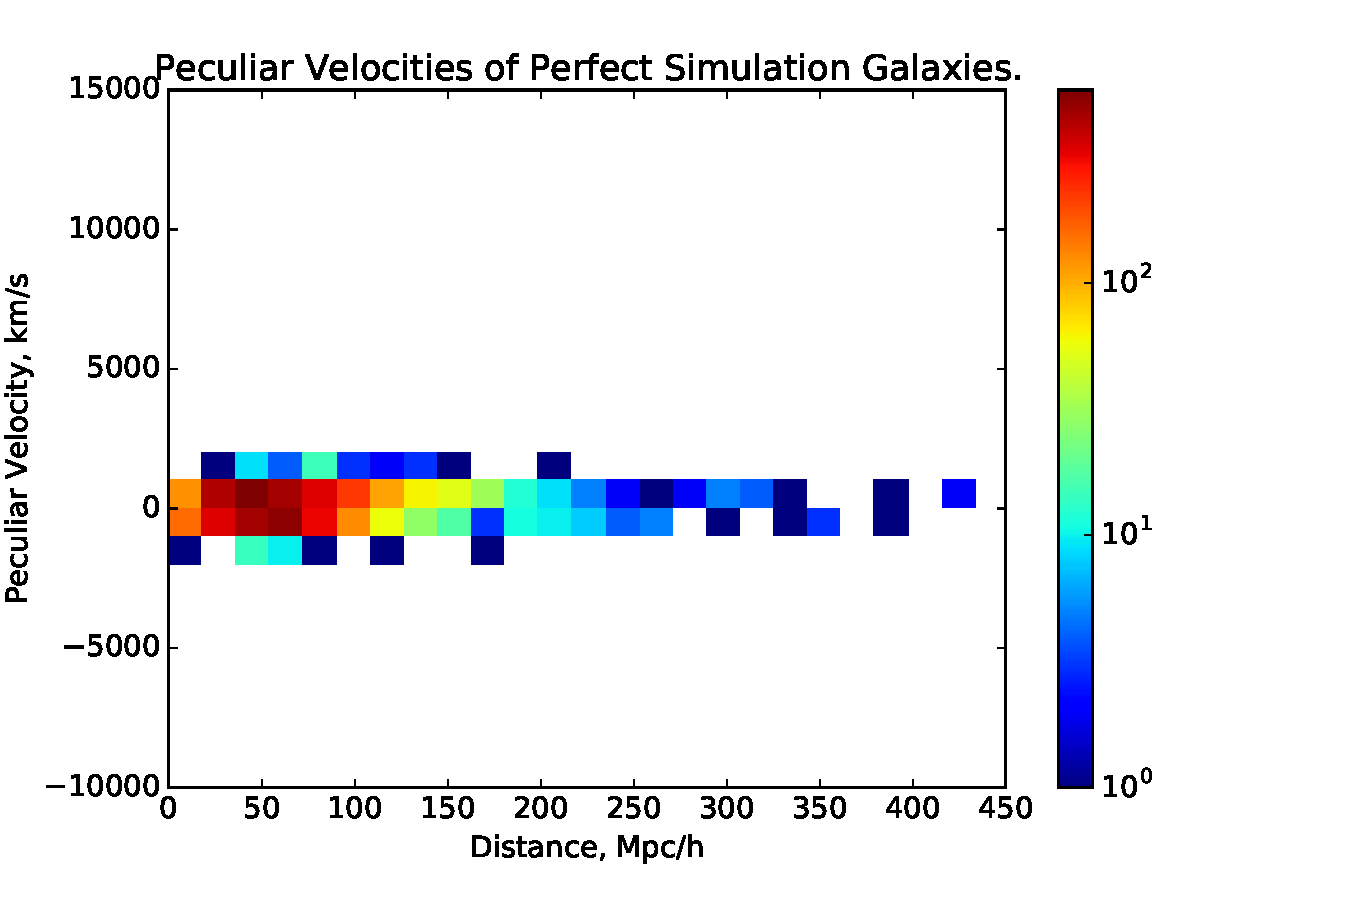
\includegraphics[scale=0.4]{perfect}
  \end{center}
\caption{\small An unperturbed sample of galaxies. The detailed structure of this sample is invisible because the scale is set for consistency with future plots. It is apparent, however, that no galaxies exist in the simulation with a peculiar velocity toward or away from us greater than 2500 km/s. Because of our perfect knowledge of these galaxies, a plot that uses redshift as distance would be exactly the same as this one, with a different x scaling factor.}
\label{fig:perfect}
\end{figure}

\begin{figure}
  \begin{center}
  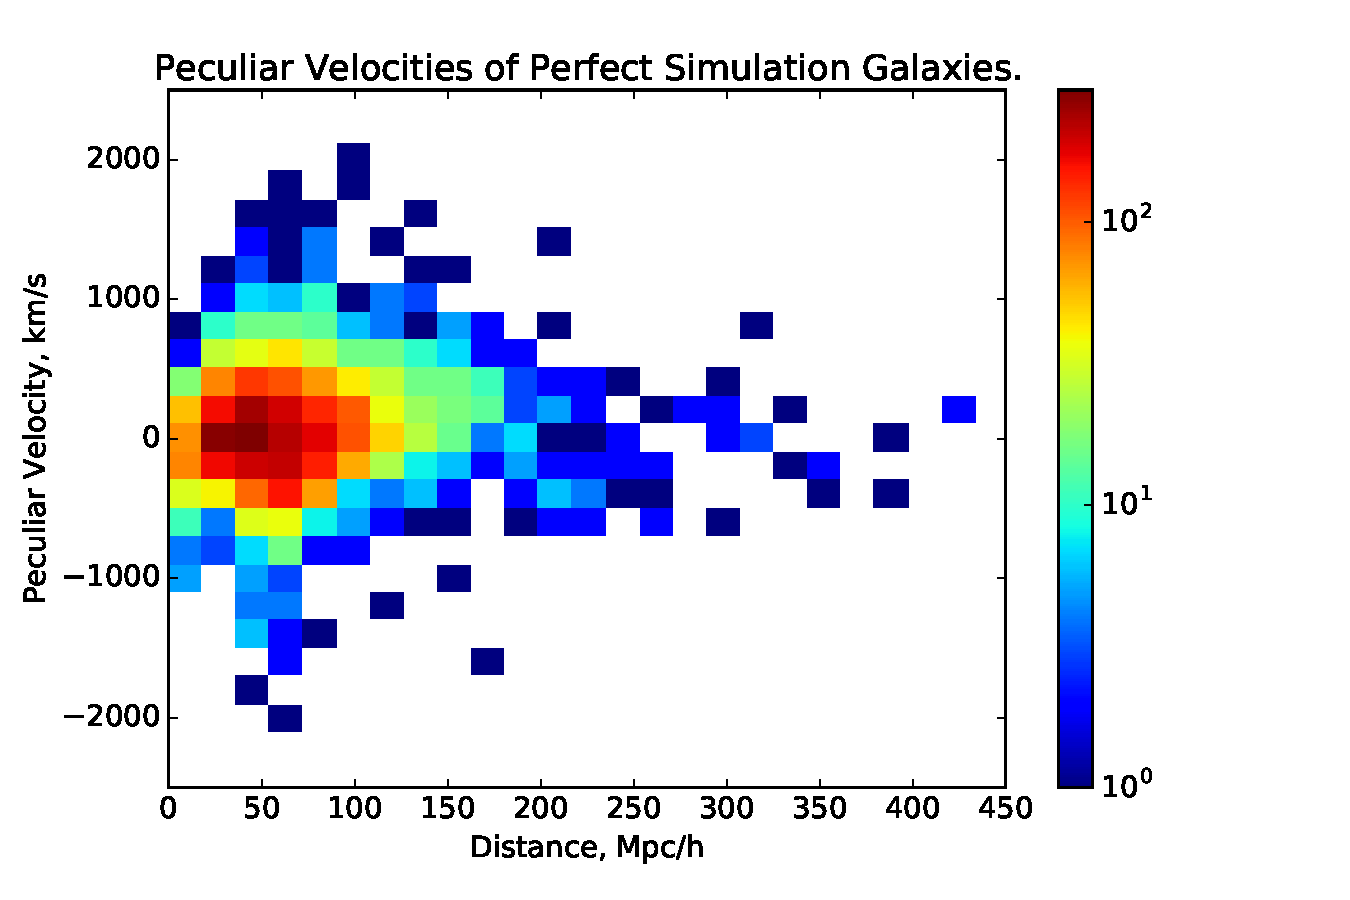
\includegraphics[scale=0.4]{perfectdetail}
  \end{center}
\caption{\small An unperturbed sample of galaxies. This plot does not have the same y-axis scaling as the rest of the plots in order to better show the structure of the unperturbed sample of galaxies.}
\label{fig:perfectzoom}
\end{figure}


The other initial sample that was used for this analysis was the COMPOSITE survey of $\approx$ 4000 galaxies. Its characteristics are shown in Fig~\ref{fig:composite}. It is apparent that there are many galaxies with much larger peculiar velocities than are seen in the simulation, due to the real problems that arise when measuring the distance to a galaxy. Fig~\ref{fig:composite} also shows the peculiar velocity plotted against redshift instead of distance, which can be more accurate at large distances.

Now we present the results from different perturbation methods. The results of the distance method are presented in Fig~\ref{fig:distance}. These plots show similar behavior to Fig~\ref{fig:composite}. I am concerned that the velocities are biased negatively when plotted against redshift. It appears that the dense region of galaxies is spread to more negative velocities at larger distances, which is an effect that we will be seeing a lot. This effect vanishes when the velocity is plotted against redshift.

The negative slope is much more exaggerated in Figs~\ref{fig:relative} and~\ref{fig:modulus}, which show, respectively, the galaxies perturbed by the relative method and the modulus method. Again, the effect vanishes when redshift is used on the x-axis, which indicates that it is an effect caused by some property of the distance calculation, not necessarily the velocity calculation.

At first I wasn't convinced that this negative slope was a problem, but I ended up exploring the parameter space a bit more and found that it is definitely a problem. I made two exaggerated plots, one using the distance method and one using the relative method. These are shown in Figs~\ref{fig:exaggerate} and~\ref{fig:exaggeratenotmod}. The bias here is absolutely terrifying.

\begin{figure}
  \begin{center}
  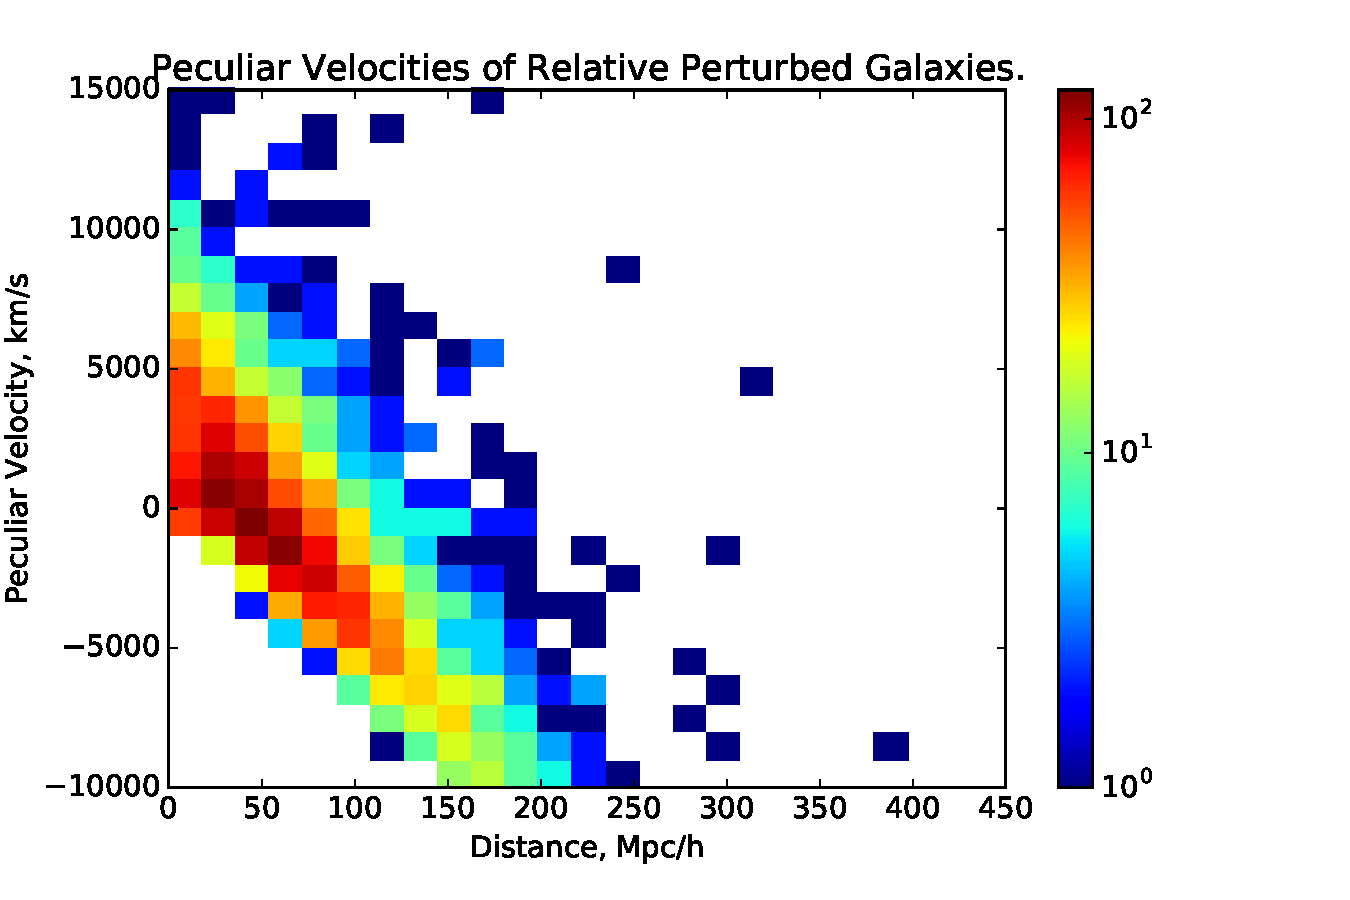
\includegraphics[scale=0.4]{exaggerate}
  \end{center}
\caption{\small The galaxy sample perturbed using the relative method with an exaggerated constant of 0.2 to show the bias.}
\label{fig:exaggerate}
\end{figure}
\begin{figure}
  \begin{center}
  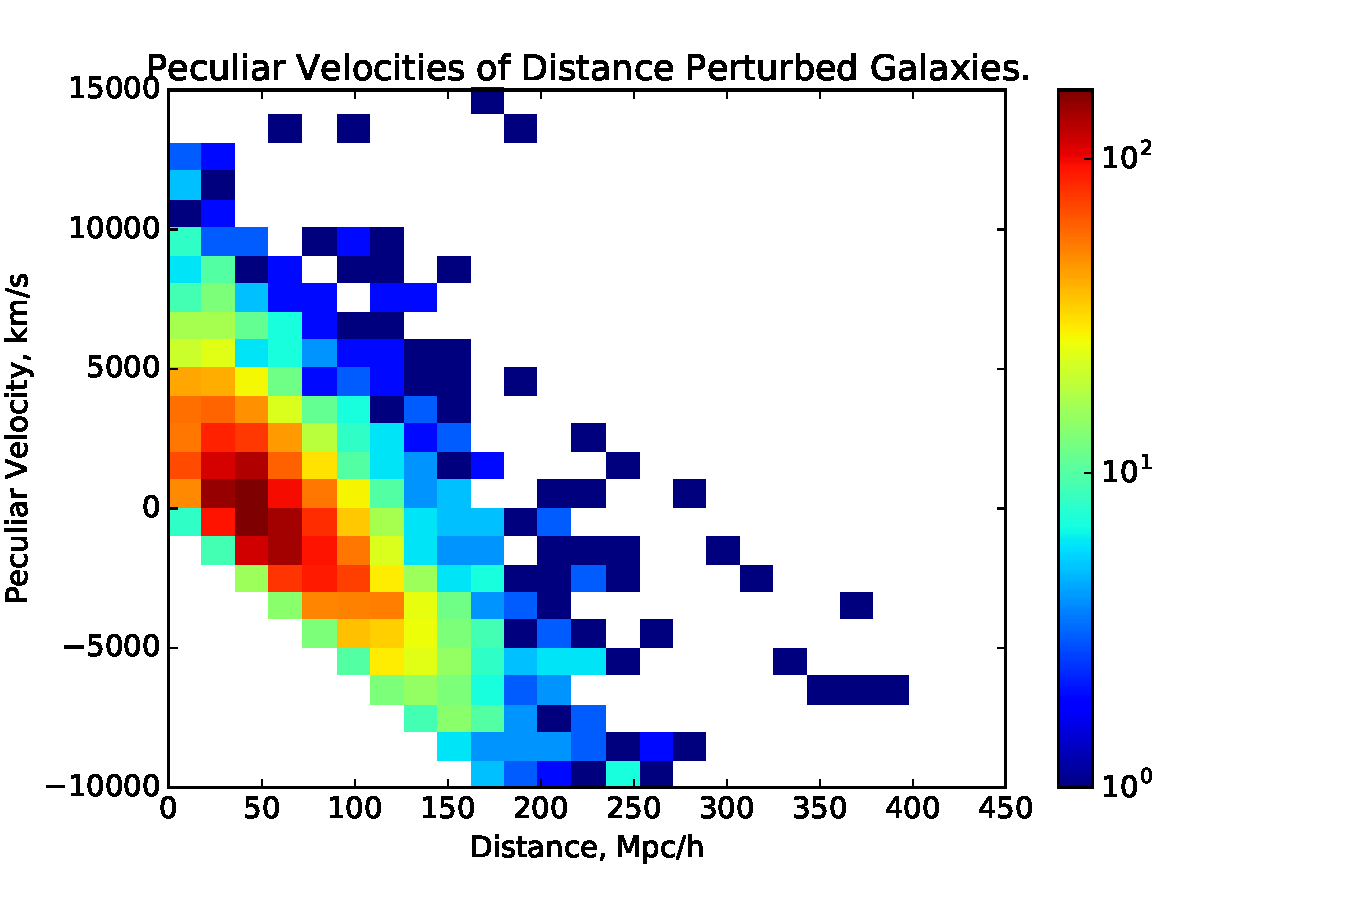
\includegraphics[scale=0.4]{exaggeratenotmod}
  \end{center}
\caption{\small The galaxy sample perturbed using the distance method with an exaggerated constant of 0.5 to show the bias.}
\label{fig:exaggeratenotmod}
\end{figure}


\begin{figure*}
\centering

  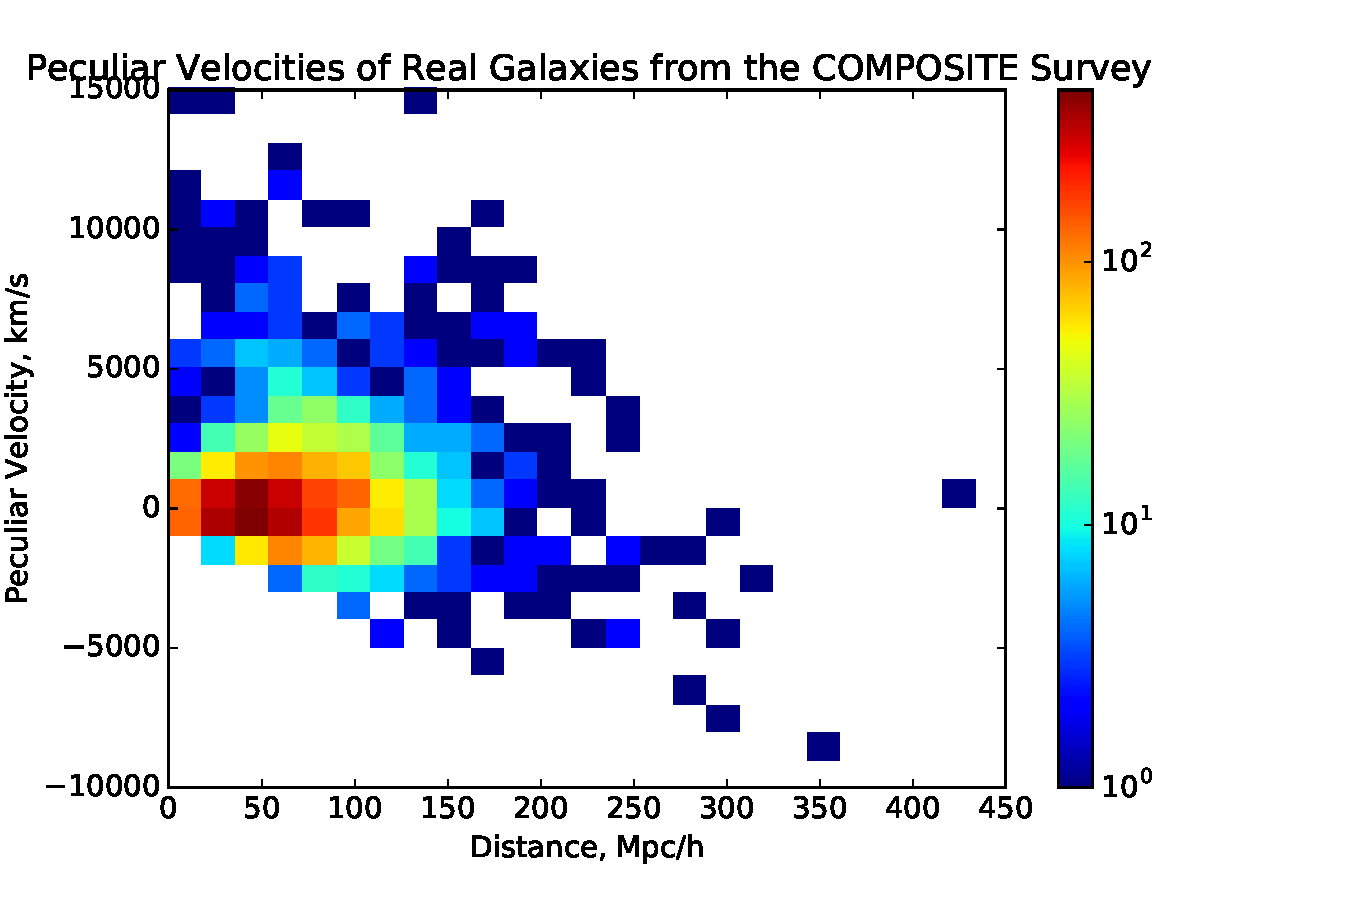
\includegraphics[scale=0.35]{composite}
\hfill
  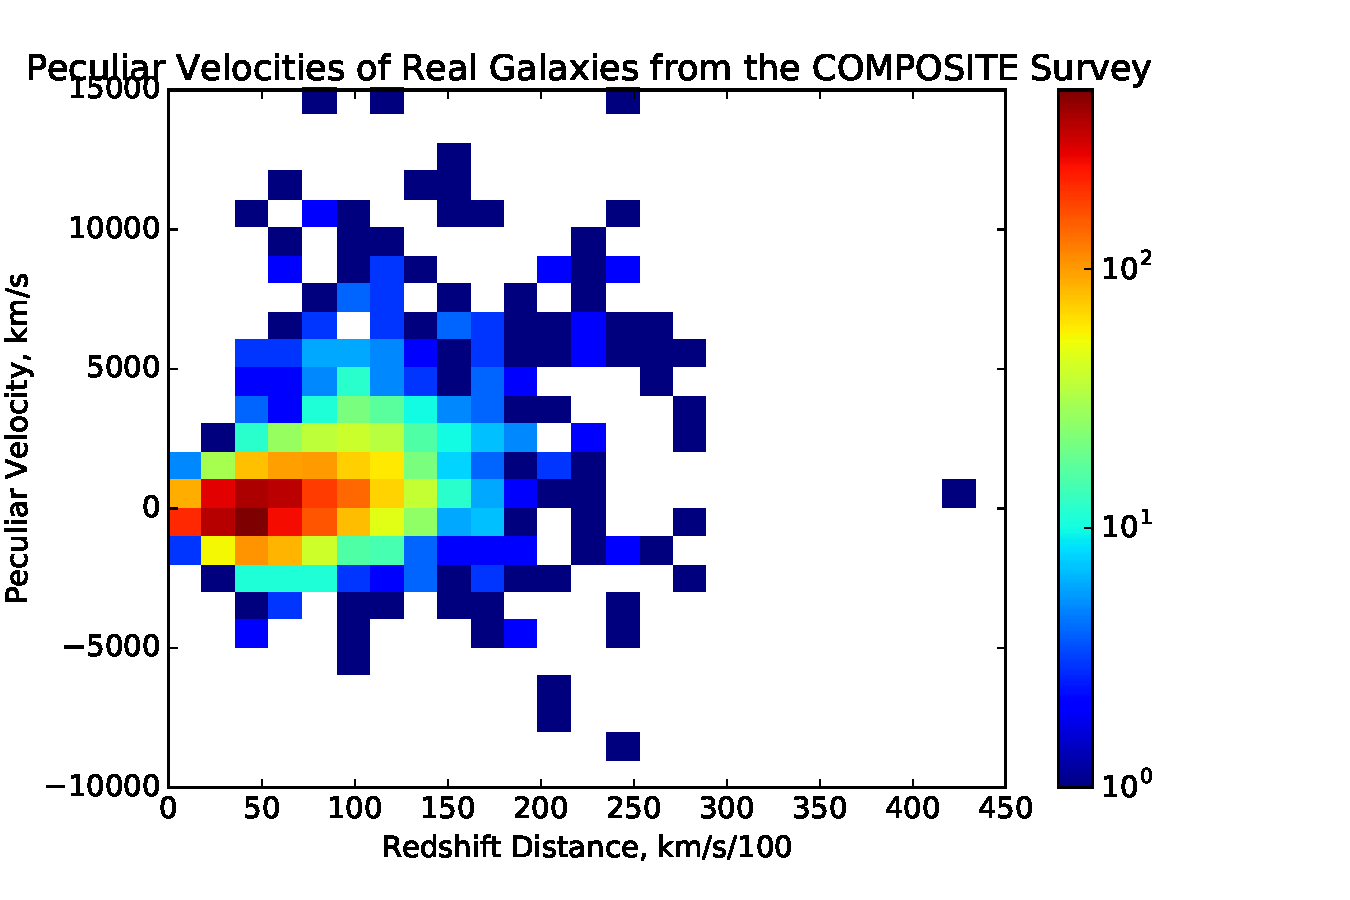
\includegraphics[scale=0.35]{compositered}
\caption{\small A real sample of galaxies. The spread in velocity is much greater than the simulation, but the simulation and sample both stay centered on zero over large distances. On the right redshift is used instead of distance to present the peculiar velocities of galaxies. At large distances, redshift is a better estimator of distance than distance is, due to the relatively low peculiar velocities of galaxies compared to cosmic expansion.}
\label{fig:composite}
\end{figure*}
\begin{figure*}
\centering
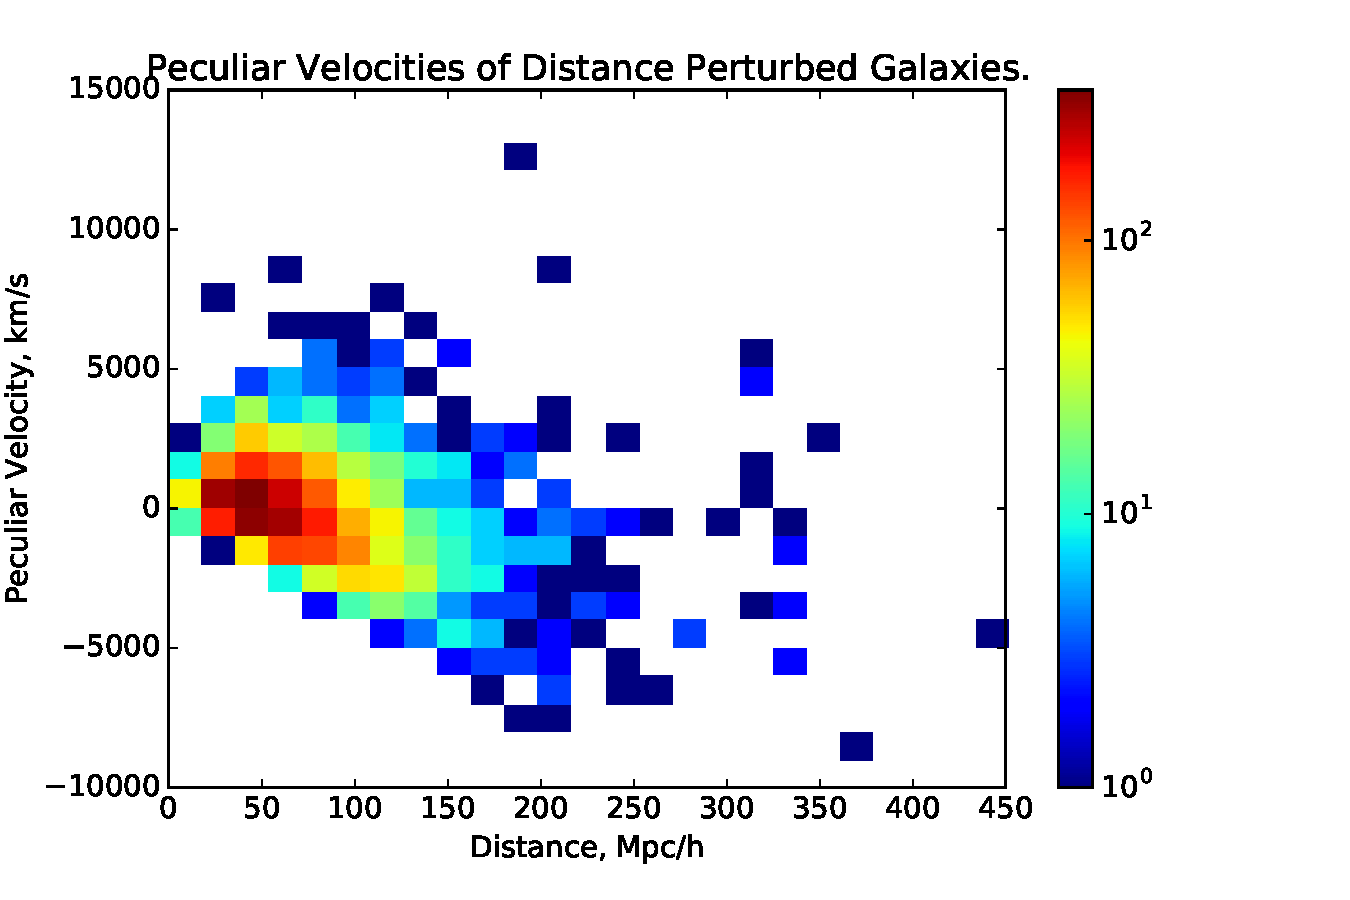
\includegraphics[scale=0.35]{distance}
\hfill
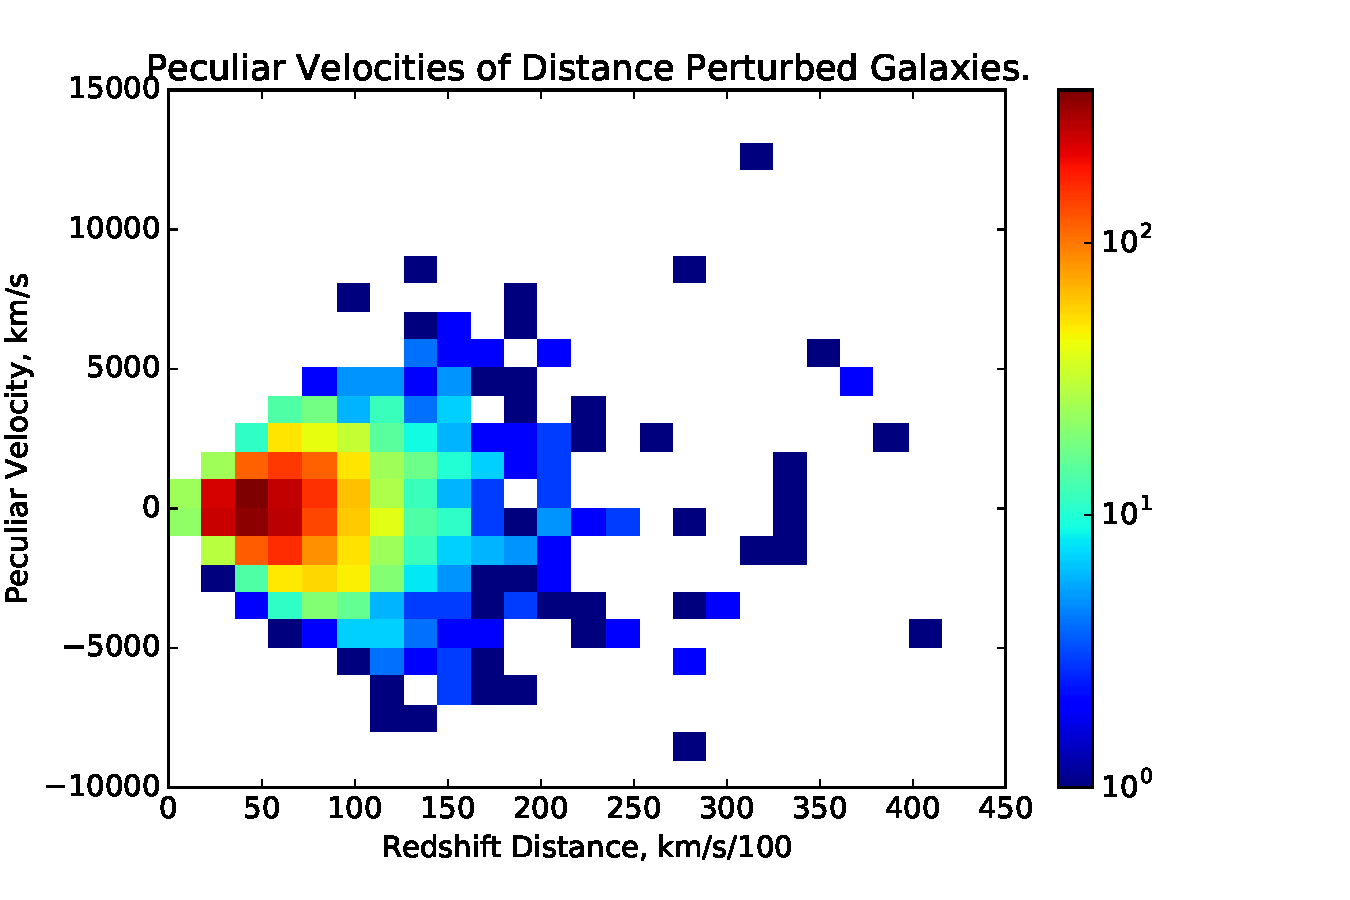
\includegraphics[scale=0.35]{distancered}
\caption{\small The perfect sample of galaxies perturbed using the distance method with $\delta d/d$ = 0.2, which is approximately the same value used in COMPOSITE. On the left the velocities are plotted against distance, on the right they're plotted using redshift as distance.}
\label{fig:distance}
\end{figure*}

\begin{figure*}
\centering
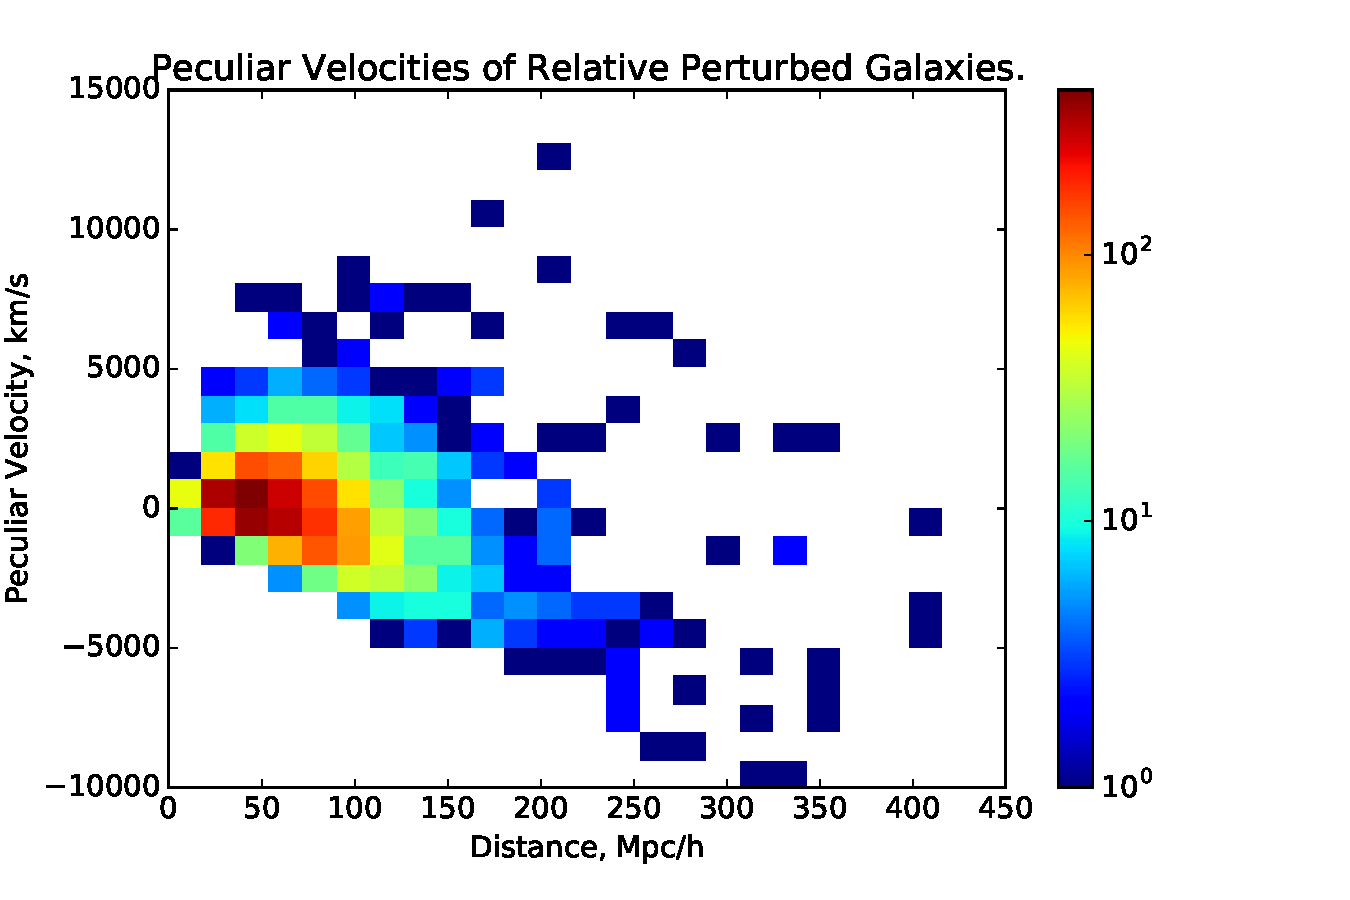
\includegraphics[scale=0.35]{relative}
\hfill
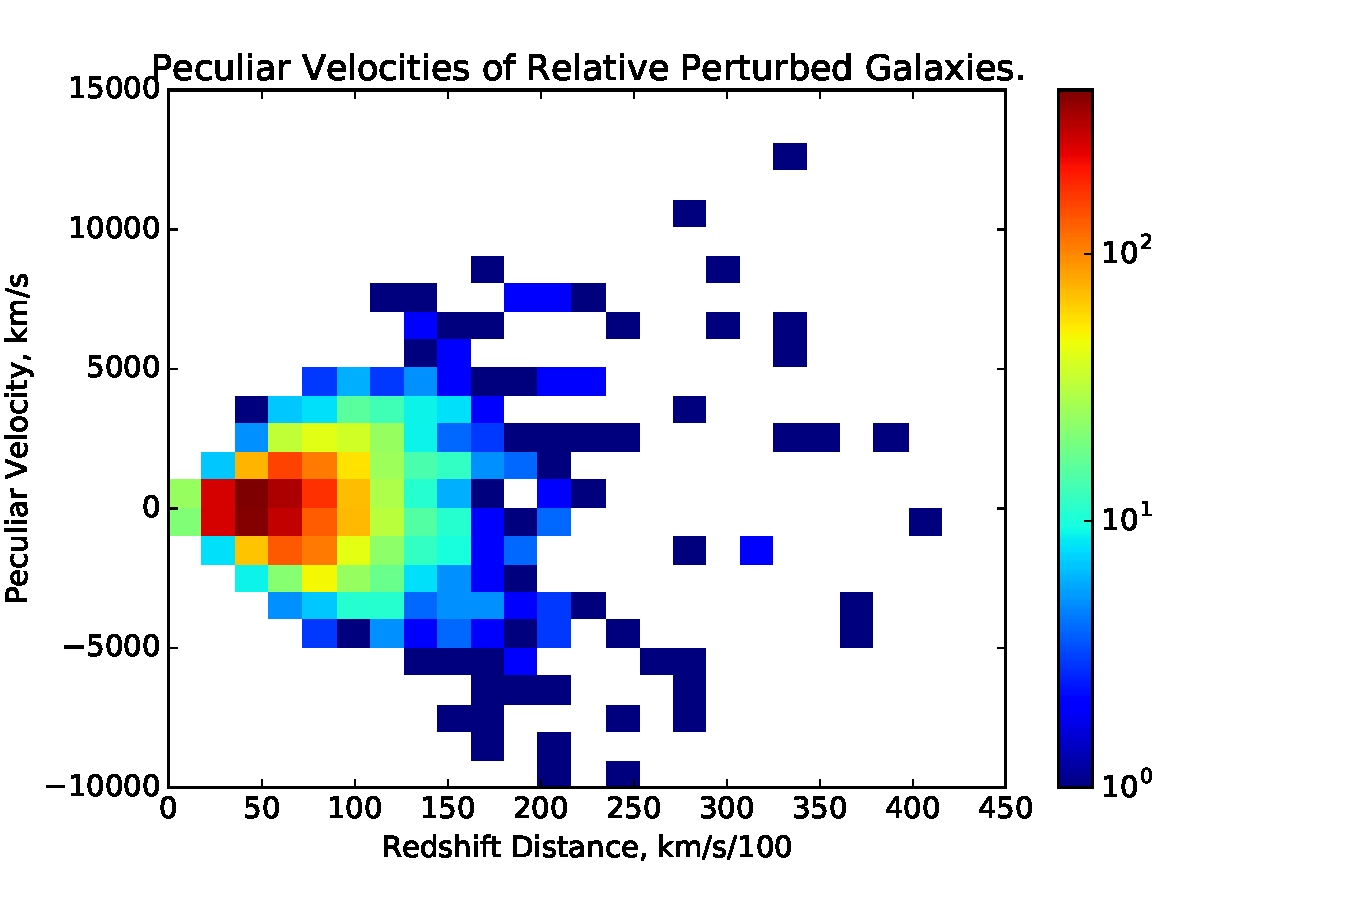
\includegraphics[scale=0.35]{relativered}
\caption{\small The perfect sample of galaxies perturbed using the relative method with $\delta \mu/\mu$ = 0.04, which is the value that ill give the same results as those in the other plots. On the left the velocities are plotted against distance, on the right they're plotted using redshift as distance.}
\label{fig:relative}
\end{figure*}
\begin{figure*}
\centering
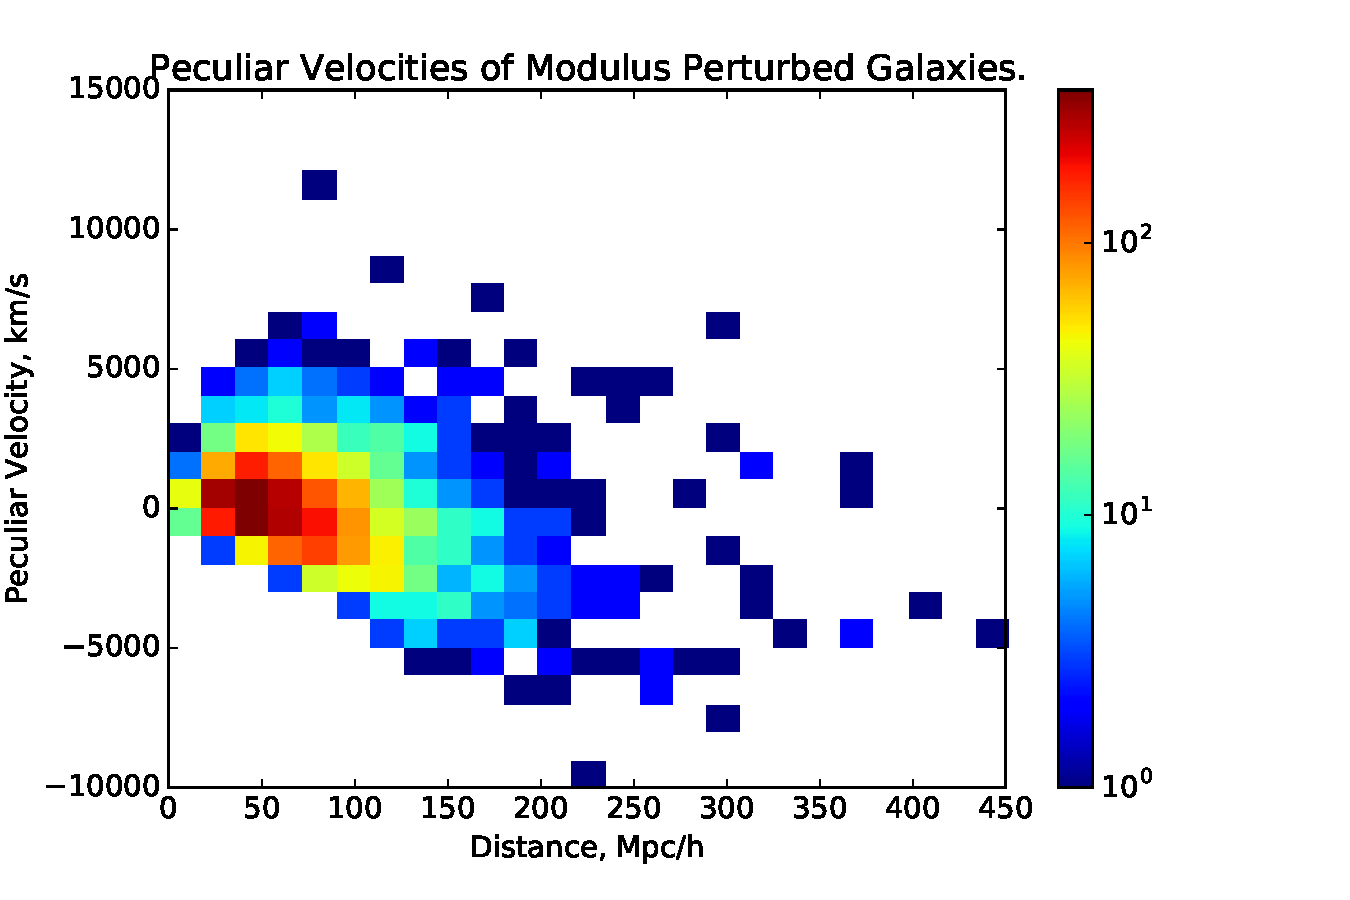
\includegraphics[scale=0.35]{modulus}
\hfill
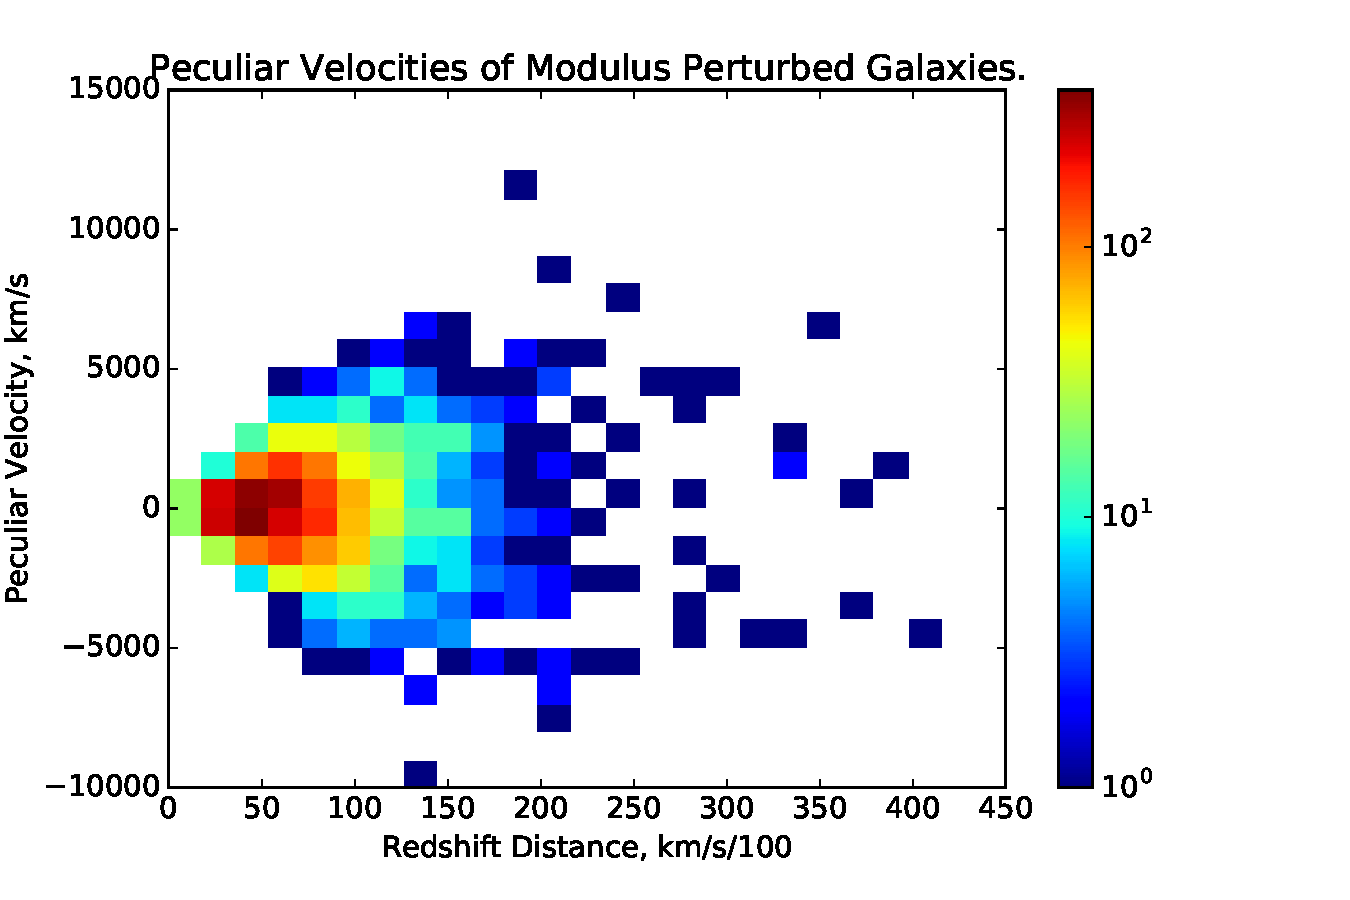
\includegraphics[scale=0.35]{modulusred}
\caption{\small The perfect sample of galaxies perturbed using the modulus method with $\delta d/d$ = 0.4, which is the value that will give the same results as those in the other plots. On the left the velocities are plotted against distance, on the right they're plotted using redshift as distance.}
\label{fig:modulus}
\end{figure*}




\section{Discussion and Conclusions}
There are obviously problems with using these methods. If the real sample was perturbed in the modulus, some corrections must have been applied to ensure that the data is not biased. The bias in these methods causes galaxies at larger distances to appear more blueshifted than is observed, and this deficiency in the perturbation method must be fixed before any meaningful results can be expected from correlations involving them. My current working guess/explanation is based off of Yuyu's idea. The peculiar velocities are estimated using an unbiased estimator, but the distances aren't. Because of that, the distances are skewed strongly, producing this negative slope in the distance plots of the relative and modulus perturbed data.

However, that isn't all because this bias appears in the distance-perturbed sample as well, which never contains a log. I have only a little experience with Malmquist bias, but it's all over the place. Could it be affecting us here?


%%%%%%%%%%%%%%%%%%%%%%%%%%%%%%%%%%%%%%%%%%%%%%%%%%%%%%%%%%%%%%%%%%%%%%
%% Finally we specify the format required for our references and the
%% name of the bibtex file where our references should be taken from.
%%%%%%%%%%%%%%%%%%%%%%%%%%%%%%%%%%%%%%%%%%%%%%%%%%%%%%%%%%%%%%%%%%%%%%
\bibliographystyle{mn2e}
\bibliography{paper}
\end{document}

%%%%%%%%%%%%%%%%%%%%%%%%%%%%%%%%%%%%%%%%%%%%%%%%%%%%%%%%%%%%%%%%%%%%%%
%% The end.
%%%%%%%%%%%%%%%%%%%%%%%%%%%%%%%%%%%%%%%%%%%%%%%%%%%%%%%%%%%%%%%%%%%%%%
